\paragraph{Objectives of the ENG subproject.}

\begin{figure}[h!]
\begin{center}
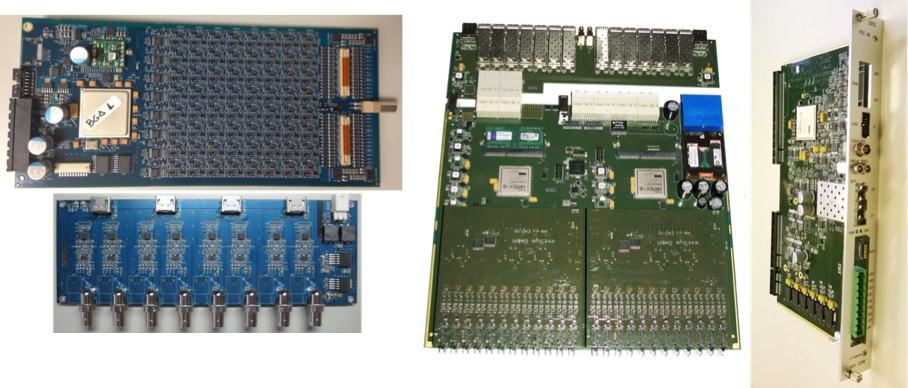
\includegraphics[width=0.9\textwidth]{img/Electronics.jpg}
\end{center}
\caption{\label{Fig:FEE} Left: Front-end boards for SiPM (top) and PMTs (bottom) for NEW and NEXT-100; right: SRS FEC modules in ATCA form factor (left) and “SRS classic” flavour (right) }
\end{figure}

The ENG subproject centralises the front-end electronics, data acquisition (DAQ), online system and slow controls of the NEW and NEXT-100 detectors. It is coordinated by the UPV.
NEXT (via the UPV team) has co-developed a new readout and DAQ concept named SRS \footcite{Toledo2011,SRS2013},for the international RD-51 collaboration at CERN. NEXT front-end modules are connected via copper links to the SRS DAQ interface modules. The CERN standard DATE environment is used as DAQ software. This brings a number of advantages, like counting on a large base of users and developers, reducing production costs and profiting from other group’s developments. SRS has been successfully used in NEXT-DEMO (PMT and SiPM readout, DAQ interface and trigger modules)\footcite{Gil2012,Herrero2012,Esteve2012} and newer versions of these modules are to be used in NEW and NEXT-100\footcite{TWEPP2014}.

The specific objectives of this sub-project are:

\begin{enumerate}

\item {\bf FEE (Front End Electronics)}. Design, fabrication and commissioning of the front-end electronics for the PMTs and the SiPMs for NEW and NEXT-100. The NP leader is the co-PI of the subproject, Prof. Francisco Toledo (UPV).
 
\item {\bf DAQ}. Design, fabrication and commissioning of the data acquisition modules for NEW and NEXT-100. The NP leader is the second co-PI of the subproject, Prof. Raul Esteve (UPV).

\item {\bf Slow control}. Design, fabrication and commissioning of the slow control for NEW and NEXT-100. The project leader is technical engineer Vicente Álvarez, under the supervision of co-IP J. Toledo. The goals are (1) monitor critical detector parameters, mostly temperature and pressure, (2) control power supplies for the sensors, detector grids and electronics and (3) implement an automatic emergency response monitor.

\item {\bf Online}. Design and commissioning of the online system for NEW and NEXT-100. Interfaces with offline, DAQ and Slow Control. The project leader is Dr. Raúl Esteve. 

\end{enumerate}